\chapter{Partcle-grid-particle}
    The basic method for generating training data which is more accessible to learning is that we will map a discrete element method(DEM) into a continuum setting use techniques from smooth particle hydrodynamics. Given a set of bodies $\delta$ and a set of contacts between these bodies $C$.

\section{Grid-Based method}
    Traditional rigid motion simulation mainly use particle-based method. However, if we want to replace traditional contact solver with deep learning model, it is hard for cnn model to recognize the original image and do learning. Grid-based methos is a good to transfer original image to a grid-cells and then use

    \begin{figure}
        \centering
        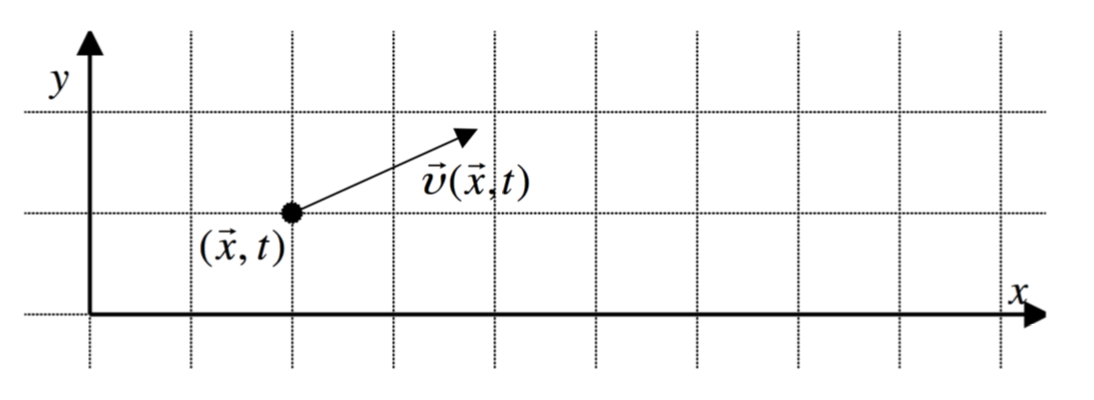
\includegraphics[scale = 0.4]{Figures/grid_method.png}
        \caption{Grid description, $retrieved from MIT(2011)$}
    \end{figure}

\section{Smoothed Particle Hydrodynamics}
    Smoothed particle hydrodynamics (SPH) was invented to simulate nonaxisymmetric phenoma in astrophysis initially. The principal idea of SPH is to treat hydrodynamics in a completely mesh-free fashion, in terms of a set of sampling particles. It turns out that the particle presentation of SPH has excellent conservation properties. Energy, linear momentum, angular momentum, mass and velocity.

    \subsection{Fundamentals}

    At the heart of SPH is a kernel interpolation method which allows any function to be expressed in terms of its values at a set of disordered points - the particles\cite{monaghan1992smoothed}. For ant field $A(\textbf{r})$, a smoothed interpolated version $A_{I}(\textbf{r})$ can be defined by a kernel $W(\textbf{r}, h)$,
    \begin{equation}
        A_{I}(\textbf{r}) = \int A({\textbf{r}}^{\prime})W(\|\textbf{r} - \textbf{r}^{\prime}\|, h)\dif\textbf{r}^{\prime}
    \end{equation}
    \begin{figure}[h!]
        \centering
        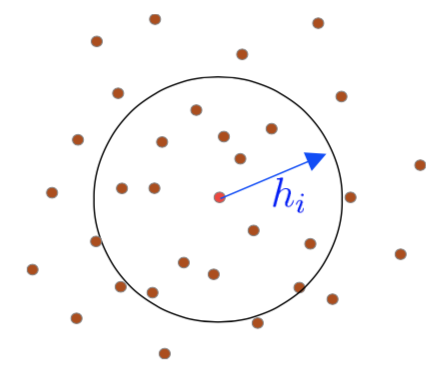
\includegraphics[scale = 0.8]{Figures/sph}
        \caption{Visilaztion of SPH}
    \end{figure}

    where the integration is over the entire space, and $W$ is an interpolating kernel with 
    \begin{equation}
        \int W(\|\textbf{r} - \textbf{r}^{\prime}\|, h)\dif \textbf{r}^{\prime} = 1
    \end{equation}
    and
    \begin{equation}
        \lim_{h\to 0} W(\|\textbf{r} - \textbf{r}^{\prime}\|, h)\dif\textbf{r}^{\prime} = \delta(\|\textbf{r} - \textbf{r}^{\prime}\|) 
    \end{equation}

    Normally, we want the kenel to be Non-negative and rotational invariant.
    \begin{equation}
        W(\|\textbf{x}_{i} - \text{x}_{j}\|, h) = W(\|\text{x}_{j} - \text{x}_{i}\|, h)
    \end{equation}

    \begin{equation}
        W(\|\textbf{r} - \textbf{r}^{\prime}\|, h) \ge 0
    \end{equation}

    For numerical work, we can use midpoint rule,
    \begin{equation}
        A_{I}(\textbf{x}) \approx A_{S}(\textbf{x}) = \sum_{i} A(\textbf{x}_{i})W(\|\textbf{x}_{i}-\textbf{x}\|, h)\Delta V_{i}
    \end{equation}
    Since $V_{i} = m_{i}/\rho _{i}$
    \begin{equation}
        A_{S}(\textbf{x}) = \sum_{i} \frac{m_{i}}{\rho_{i}} A(\textbf{x}_{i})W(\|\textbf{x}_{i}-\textbf{x}\|, h)
    \end{equation}

    The default, gradient and Laplacian of $A$ are:
    \begin{equation}
        \begin{aligned}
        \nabla A_{S}(\textbf{x}) &= \sum_{i} \frac{m_{i}}{\rho_{i}} A(\textbf{x}_{i})\nabla W(\|\textbf{x}_{i}-\textbf{x}\|, h) \\
        \nabla^{2} A_{S}(\textbf{x}) &= \sum_{i} \frac{m_{i}}{\rho_{i}} A(\textbf{x}_{i})\nabla^{2} W(\|\textbf{x}_{i}-\textbf{x}\|, h)
        \end{aligned}
        \label{eq_all}
    \end{equation}

    \subsection{Kernels}
    Smoothing kernels functions are one of the most important points in SPH. Stability, accurancy and speed of the whole method depends on these fuctions. Different kernels are being used for different purposes. One possibilyty for $W$ is a Gaussian. However, most current SPH implementations are based on kernels with finite support. We mainly introduce gaussian, poly6 and spicky kernel here. And compare the different kernels and their property.

    \subsubsection{Poly6}
    The kernel is also known as the 6th degree polynomial kernel.
    \begin{equation}
        W_{poly6}(\textbf{r}, h) = \frac{315}{64\pi h^{9}}
            \begin{cases}
                (h^2 - \|\textbf{r}\|^2)^3 & 0\le\|\texfbf{r}\|\le h \\
                0 & Otherwise
            \end{cases}
    \end{equation}

    Then, the gradient of this kernel function can be
    \begin{equation}
        \nabla W_{poly6}(\textbf{r}, h) = - \frac{945}{32\pi h^9}
            \begin{cases}
                \textbf{r}(h^2 - \|\textbf{r}\|^2)^2 & 0\le\|\texfbf{r}\|\le h \\
                0 & Otherwise \\
            \end{cases}
    \end{equation}

    The laplacian of this kenel can be expressed by, 
    \begin{equation}
        \nabla^2 W_{poly6}(\textbf{r}, h) = - \frac{945}{16\pi h^9}
            \begin{cases}
                (h^2 - \|\textbf{r}\|^2)(3h^2-7\|\textbf{r}\|^2) & 0\le\|\texfbf{r}\|\le h \\
                0 & Otherwise \\
            \end{cases}
    \end{equation}

    \subsubsection{Spicky}

    The kernel proposed by Desbrum\cite{desbrun1996smoothed}
    \begin{equation}
        W_{spiky}(\textbf{r}, h) = \frac{15}{\pi h^6}
            \begin{cases}
                (h - \|\textbf{r}\|)^3 & 0\le\|\texfbf{r}\|\le h \\
                0 & Otherwise \\
            \end{cases}
    \end{equation}

    Then, the gradient of spiky kernel can be described by,
    \begin{equation}
        \nabla W_{spiky}(\textbf{r}, h) = -\frac{45 \textbf{r}}{\pi h^6 \|\textbf{r}\|}
            \begin{cases}
                (h - \|\textbf{r}\|)^2 & 0\le\|\texfbf{r}\|\le h \\
                0 & Otherwise \\
            \end{cases}
    \end{equation}
     The laplacian of spiky can be expressed by,
     \begin{equation}
        \nabla^2 W_{spiky}(\textbf{r}, h) = \frac{90}{\pi h^6}
            \begin{cases}
                h - \|\textbf{r}\| & 0\le\|\texfbf{r}\|\le h \\
                0 & Otherwise \\
            \end{cases}
    \end{equation}

    \begin{figure}[h!]
        \centering
        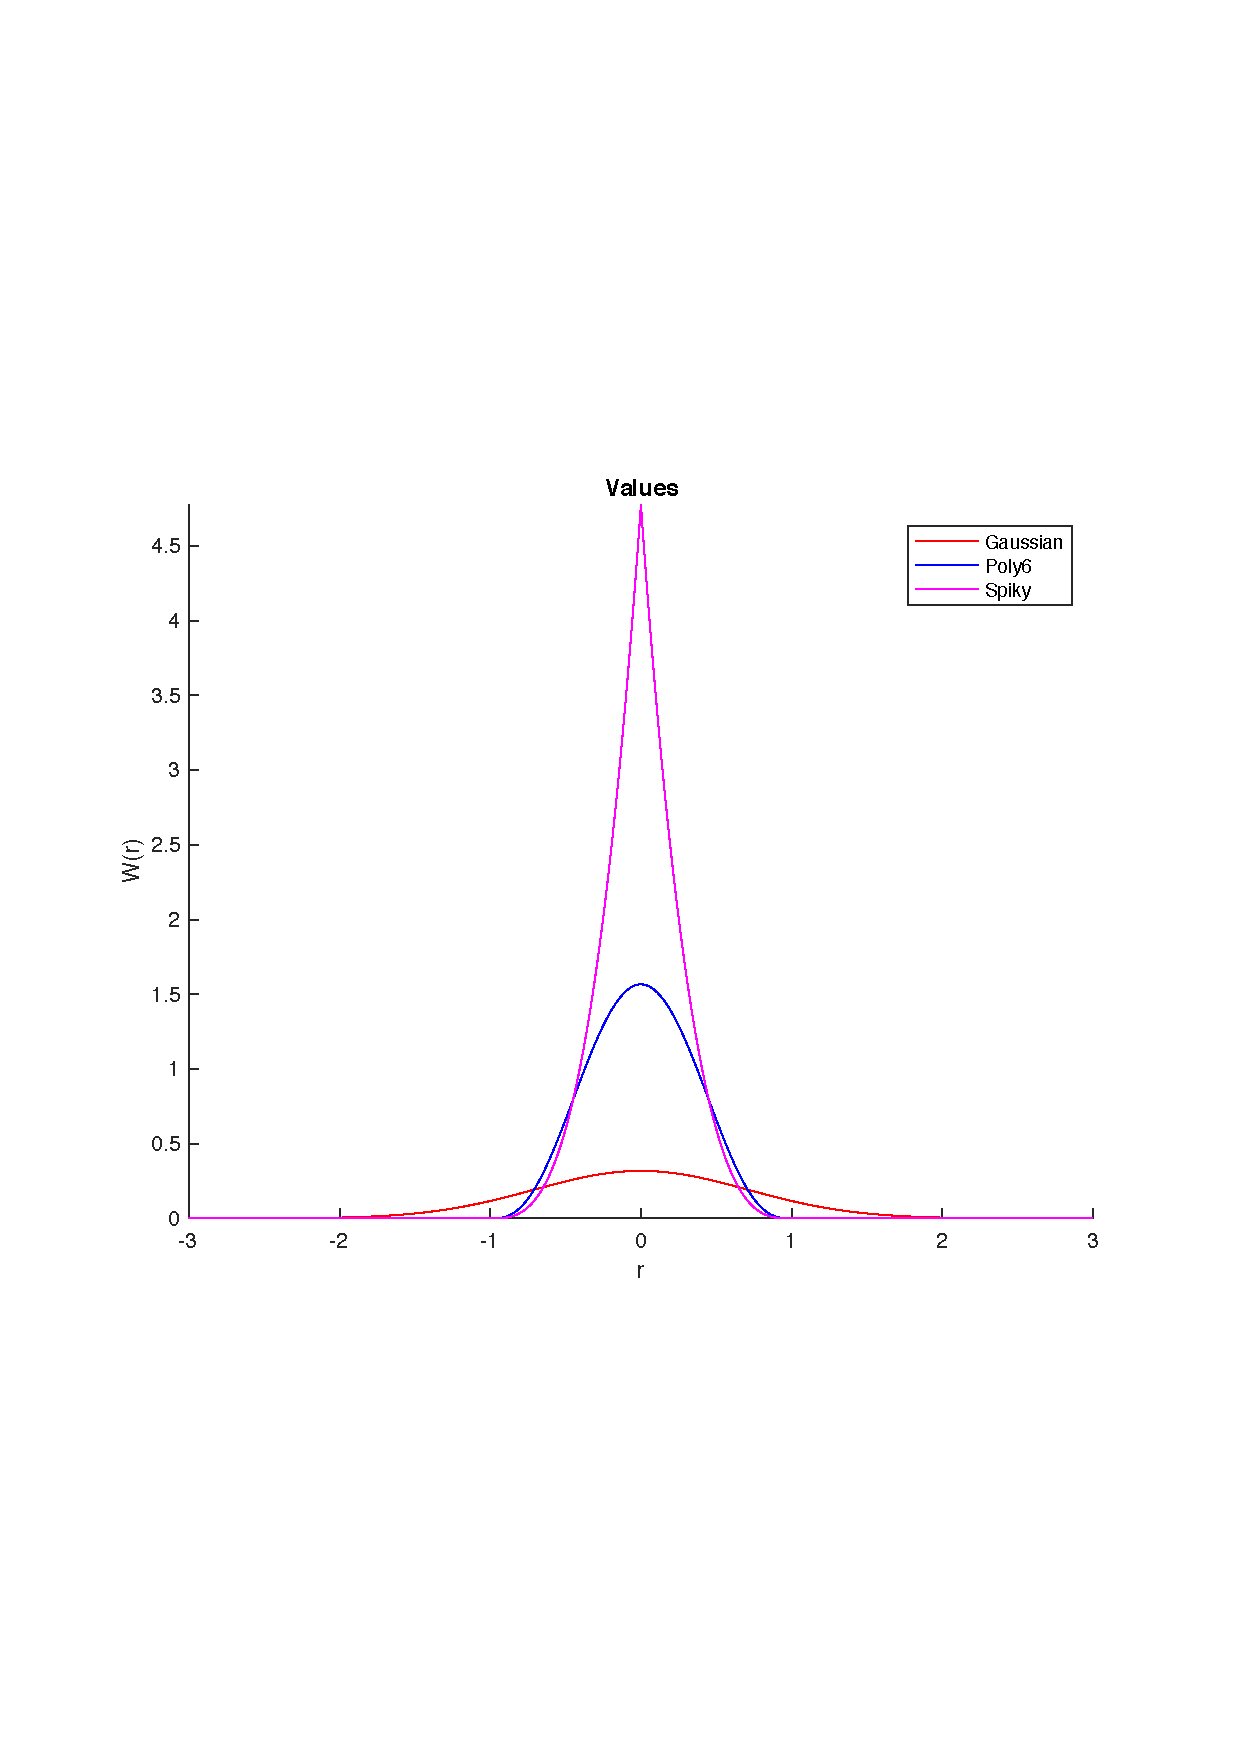
\includegraphics[scale = 0.2]{Figures/kernels}
        \caption{Comparation of different kernels, we set smoothing length $h = 1$ here.}
    \end{figure}

    \begin{figure}[h!]
        \centering
        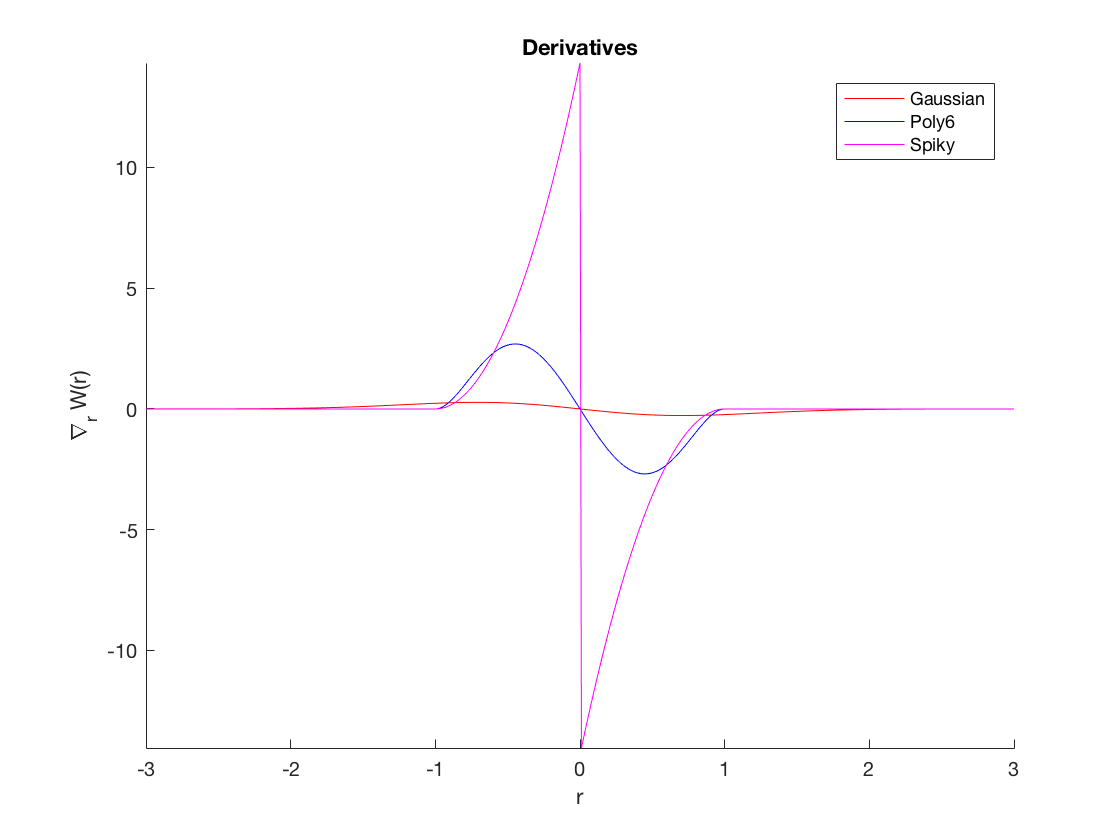
\includegraphics[scale = 0.2]{Figures/kernels_de}
        \caption{Comparation of gradient of different kernels, we set $h = 1$ here. }
    \end{figure}

    \subsection{Grid size and smoothing length}

    The grid should be also fine enough to capture the variation in our simulation. In our case, it is reasonale to have a grid fine enough such that no two contact points are mapped into the same cell. \\

    Smoothing length, $h$, is one of the most important parameters that affects the whole SPH method by changing the kernal value results abd neigbor searching results. Too small or too big values might cause lose essencail information in the simulation.

    \subsection{Neignbor Search}
    Neighbor search is one of the most crucial procedures in SPH method considersing all interpolation equations, $A(\textbf{r})$, needs the neighbor list for every particle (refer to equation \eqref{eq_all})


\section{Grid to particle}
    \subsection{interpolation}

\section{Conclution}